\documentclass[12pt,a4paper]{article}
\usepackage[utf8]{inputenc}
\usepackage[T1]{fontenc}
\usepackage[brazil]{babel}
\usepackage[margin=2.5cm]{geometry}
\usepackage{booktabs}
\usepackage{amsmath,amssymb}
\usepackage{caption}
\usepackage{graphicx}
\usepackage{setspace}
\usepackage{indentfirst}
\usepackage{fancyhdr}
\usepackage[hidelinks]{hyperref}
\graphicspath{{docs/}}

\captionsetup{font=small,labelsep=colon}
\onehalfspacing

\pagestyle{fancy}
\fancyhf{}
\fancyhead[L]{\footnotesize Determinantes e previsibilidade dos pesos de ações em fundos}
\fancyhead[R]{\footnotesize J. P. Zangrandi}
\fancyfoot[C]{\thepage}
\renewcommand{\headrulewidth}{0.4pt}

\begin{document}

%==================== CAPA ====================
\thispagestyle{empty}
\begin{center}
{\large FUNDAÇÃO GETÚLIO VARGAS}\\[2pt]
{\large ESCOLA DE ECONOMIA DE SÃO PAULO}\\[16pt]
{\normalsize Graduação em Economia}

\vspace{3.5cm}

{\large João Paulo Zangrandi}

\vspace{3.0cm}

{\Large Estudo sobre a Demanda Institucional por Ativos Financeiros}

\vspace{3.0cm}

\begin{flushright}
\begin{minipage}{0.62\textwidth}
\small\setstretch{1.15}
Monografia I apresentada à Escola de Economia de São Paulo da Fundação Getúlio
Vargas como requisito da disciplina Monografia I.
\\[10pt]
Orientador: Prof.\ Maurício Ferraresi Junior.
\end{minipage}
\end{flushright}

\vfill

{\normalsize São Paulo}\\
{\normalsize 2026}
\end{center}

\newpage

%==================== RESUMO / ABSTRACT ====================
\thispagestyle{fancy}
\begin{center}{\large Resumo}\end{center}
\noindent
Este trabalho estuda os determinantes da demanda dos fundos do Itaú entre 2016 a 2021 e a
capacidade desses determinantes de prever as escolhas futuras desses fundos. O foco inicial
foi a demanda pela ação da Vale no mercado brasileiro. A abordagem segue a lógica de um
sistema de demanda institucional: a cada mês, o peso é regredido por mínimos quadrados sobre
características de cada fundo, e os coeficientes são lidos como um fator latente que varia no
tempo. Diferentemente de Koijen e Yogo (2019), fixa-se o ativo e faz-se o peso depender do
perfil do fundo. O peso é explicado pelo tamanho do fundo, pelo número de cotistas e pela
classificação como fundo de cotas, com sinais estáveis nos 72 meses; a decisão de ter a ação
tem sinais opostos à de quanto carregar. Nenhum modelo estrutural supera inicialmente a
previsão de repetir o último peso. O trabalho especifica um modelo de ajuste parcial e discute
o viés de atenuação.

\smallskip
\noindent Palavras-chave: sistema de demanda; fundos de investimento; pesos de carteira;
fator latente dinâmico; previsão; mercado acionário brasileiro.

\bigskip
\begin{center}{\large Abstract}\end{center}
\noindent
This paper studies the determinants of demand of Itaú funds between 2016 and 2021 and the
capacity of these determinants to predict the future choices of these funds. The initial focus
was the demand for the Vale stock in the Brazilian market. The approach follows the logic of
an institutional demand system: each month, the weight is regressed by ordinary least squares
on characteristics of each fund, and the coefficients are read as a latent factor that varies
over time. Unlike Koijen and Yogo (2019), the asset is fixed and the weight is made to depend
on the fund profile. The weight is explained by fund size, by the number of shareholders, and
by the classification as a fund of funds, with stable signs across the 72 months; the decision
to hold the stock has signs opposite to the decision of how much to hold. No structural model
initially beats the forecast of repeating the last weight. The paper specifies a partial
adjustment model and discusses the attenuation bias.

\smallskip
\noindent Keywords: demand system; mutual funds; portfolio weights; time-varying latent
factor; forecasting; Brazilian equity market.

\newpage
\thispagestyle{fancy}
\tableofcontents
\newpage

%==================== 1. INTRODUÇÃO ====================
\section{Introdução}

A composição das carteiras dos fundos de investimento é uma das informações mais ricas e ao
mesmo tempo menos exploradas do mercado de capitais brasileiro. Quando um fundo decide quanto
de cada ação carregar, ele revela, ainda que parcialmente, a sua demanda por aquele papel.
Olhar para todos os fundos de uma mesma gestora ao mesmo tempo equivale, então, a observar um
grande conjunto de decisões de demanda tomadas sob informações e incentivos parecidos, o que
torna possível investigar de forma organizada duas perguntas. A primeira é quais
características de um fundo explicam o peso que ele atribui a uma ação. A segunda é se esse peso
pode ser previsto de um mês para o outro.

Para tornar o problema tratável, este trabalho concentra-se em um caso concreto. Estuda-se o
peso da ação VALE3 nas carteiras dos fundos das três gestoras do grupo Itaú, a saber, Itaú
Asset Management, Itaú DTVM e Itaú Unibanco, no período de 2016 a 2021. A escolha do peso como
variável de interesse, em vez do valor financeiro ou do número de ações, é deliberada. O peso
é limitado entre zero e um, o que o torna mais simples de comparar; é comparável entre fundos
de tamanhos muito distintos; e corresponde diretamente à noção de demanda relativa que organiza
os modelos de demanda por ativos. Esse mesmo limite entre zero e um, contudo, impõe uma
exigência sobre a forma funcional.

O arcabouço teórico usado para este trabalho é o sistema de demanda de Koijen e Yogo (2019),
que propõem tratar os preços dos ativos como resultado das demandas de investidores que
escolhem suas carteiras em função das características dos ativos. A principal vantagem dessa
abordagem é reduzir um problema de dimensão muito alta, com milhares de ativos e investidores,
a um número pequeno de parâmetros associados às características.

É necessário, porém, ser preciso quanto ao ponto em que este trabalho se afasta daquele
modelo. Em Koijen e Yogo, a demanda do investidor $i$ pelo ativo $n$ é função das
características do ativo, e o vetor de sensibilidades varia por investidor; a identificação
enfrenta a endogeneidade entre preço e demanda por meio de um instrumento construído a partir
das características dos demais investidores. Aqui a lógica é, em sentido estrito, invertida em
três aspectos.

Primeiro, o ativo é fixo, VALE3, e o que varia entre observações são as características do
fundo. Segundo, a sensibilidade das escolhas em VALE3 em relação às características de cada
fundo é comum a todos os fundos em cada mês, em vez de específica ao investidor. Terceiro, não
há modelagem do canal preço-demanda nem estimação de elasticidade. O que se estima é, portanto,
um sistema de demanda institucional na forma reduzida através das quantidades escolhidas: como
o peso de uma ação reage ao perfil dos fundos que a carregam. A justificativa econômica para
esperar tal dependência está em restrições de mandato, de liquidez e de diversificação que
distinguem fundos grandes de pequenos, fundos de muitos cotistas de fundos concentrados, e
fundos de cotas de fundos que investem diretamente em ações.

Em linha próxima, Gabaix e Koijen (2021) argumentam que os mercados são inelásticos, de modo
que fluxos de demanda têm efeito expressivo sobre preços. Essa hipótese reforça o interesse
geral em medir a demanda dos investidores institucionais, mas convém registrar que ela diz
respeito ao efeito de fluxos sobre preços, canal que este trabalho não estima. A referência
serve, portanto, para motivar a relevância de observar diretamente a demanda, e não como
evidência da inelasticidade aqui medida.

Do ponto de vista do método, a estratégia adotada é estimar os coeficientes da regressão mês a
mês e, em seguida, resumir a média e a variação desses coeficientes ao longo do tempo,
procedimento consagrado por Fama e MacBeth (1973) na literatura empírica de apreçamento de
ativos. Uma ressalva técnica acompanha esse procedimento desde já: o erro padrão de
Fama-MacBeth pressupõe coeficientes serialmente independentes, e a própria amostra mostra que
não é esse o caso; por isso os erros padrão são corrigidos para autocorrelação, como detalhado
na Seção 3 e aplicado na Seção 4. Quando a sequência de coeficientes passa a ser tratada como
uma série temporal, e quando se procura separar o sinal persistente do ruído de estimação de
cada mês, recorre-se à ideia de modelos de espaço de estados e ao filtro de Kalman,
apresentados de forma didática por Harvey (1989). Como uma das características empregadas é o
fluxo líquido dos fundos, é pertinente a literatura que liga fluxos à negociação: Coval e
Stafford (2007) mostram que fundos pressionados por resgates são forçados a vender e que
entradas levam a compras, com efeito sobre preços, e Lou (2012) relaciona fluxos à
previsibilidade de retornos. O fluxo é incluído precisamente para testar se ele ajuda a
antecipar a variação do peso da ação na carteira.

A pergunta de previsão é avaliada contra uma referência exigente, a previsão ingênua que apenas
repete o último valor observado, seguindo a disciplina usual dessa literatura, segundo a qual
um modelo só interessa se conseguir superar essa regra simples. No caso brasileiro, a evidência
sobre demanda por ativos a partir de carteiras de fundos é escassa, o que motiva organizar, de
forma reprodutível e a partir das bases públicas da Comissão de Valores Mobiliários, um painel
de pesos de carteira e um conjunto de exercícios de explicação e de previsão.

O resultado central que emerge tem dois lados. Para explicar o peso, as características
funcionam bem: fundos maiores carregam menos VALE3 em peso, fundos com mais cotistas carregam
mais, e os fundos de cotas têm posição direta menor, com sinais que se repetem em todos os
meses da amostra. Para prever, no entanto, nenhum dos modelos estruturais testados supera a
regra simples de repetir o último peso. Em outras palavras, no nível de cada fundo o peso é
muito persistente e comporta-se quase como um passeio aleatório. Esse contraste, entre um bom
poder de explicação e um fraco poder de previsão de curto prazo, é o que se considera o achado
principal desta entrega.

O restante do texto está organizado da seguinte forma. A Seção 2 descreve os dados e seu
tratamento. A Seção 3 detalha a metodologia, incluindo a forma funcional adequada ao suporte da
variável, a correção de erros padrão e a especificação do modelo de ajuste parcial que será
estimado na continuação do trabalho. A Seção 4 apresenta e interpreta os resultados, com
atenção particular às tabelas e à figura. A Seção 5 conclui e aponta a agenda futura.

%==================== 2. DADOS ====================
\section{Dados}

A base empírica reúne duas fontes principais da Comissão de Valores Mobiliários e uma fonte de
mercado para o preço da ação. A primeira fonte é a composição consolidada das carteiras dos
fundos, de frequência mensal, da qual se extrai o peso de VALE3 em cada fundo, sempre tomado
como posição direta no ativo identificado como VALE ON. A segunda é a série histórica diária
dos fundos, da qual se obtêm o patrimônio líquido, o número de cotistas e a informação de o
fundo ser ou não um fundo de investimento em cotas. A captação líquida, isto é, a captação
menos os resgates, é obtida do Informe Diário da mesma Comissão, que é a base de origem da série
histórica e a única que registra os resgates. O preço e o beta de VALE3 são calculados a partir
de cotações de mercado.

O tratamento dos dados privilegia a consistência e a ausência de informação espúria. O nome da
gestora é padronizado, removendo acentuação, caixa e sufixos, de modo a reunir corretamente as
três variações do grupo Itaú. Linhas exatamente duplicadas da base de composição, que a
Comissão ocasionalmente repete, são colapsadas. Pesos negativos, que aparecem apenas como
resíduos contábeis de magnitude desprezível, são descartados, pois não têm interpretação como
participação na carteira. Após montar o painel, verifica-se que não há par de fundo e mês
repetido. Os fundos exclusivos são retirados por meio de um critério simples, mantendo-se apenas
as observações com mais de três cotistas, uma vez que fundos com um ou dois cotistas refletem
decisões de um único investidor e não a demanda difusa que se quer estudar. O limiar de três
cotistas é, reconhecidamente, uma convenção, e a continuação do trabalho reportará a
sensibilidade dos resultados a esse corte. O casamento entre a base diária e a base mensal é
feito pelo dia exato da competência, sem perda de observações.

Dois cuidados de validação merecem registro. Primeiro, a captação líquida obtida do Informe
Diário foi confrontada com a informação correspondente da série histórica, e a coincidência é
quase perfeita, com mais de noventa e nove por cento dos pares de fundo e mês batendo ao
centavo; as poucas divergências decorrem de diferenças entre as duas séries da própria Comissão,
e não de erro de processamento. Segundo, o preço de VALE3 foi conferido contra o fechamento
oficial da bolsa nas datas de referência utilizadas, sem diferença relevante. O beta é calculado
como a razão entre a covariância dos retornos da ação e do Ibovespa e a variância dos retornos
do índice, em janela móvel de duzentos e cinquenta e dois pregões.

Aplicados esses critérios, o painel cobre os 72 meses entre 2016 e 2021 e abrange as três
gestoras do grupo Itaú. O painel completo de fundos que detêm a ação reúne 26.123 observações de
fundo por mês, distribuídas em 623 fundos. A amostra que entra nas regressões de explicação,
restrita aos fundos com mais de três cotistas e com fluxo disponível, contém 11.413 observações
de fundo por mês, provenientes de 307 fundos, das quais cerca de três quartos correspondem a
fundos de cotas. A Tabela~\ref{tab:desc} resume as variáveis nessa amostra.

\begin{table}[h]\centering\small
\caption{Estatísticas descritivas da amostra de regressão (11.413 observações de fundo por mês, 2016--2021).}
\label{tab:desc}
\begin{tabular}{@{}lrrrrr@{}}
\toprule
Variável & Média & Desvio-padrão & Mediana & Mínimo & Máximo \\
\midrule
Peso de VALE3 (\%)            & $2{,}87$ & $3{,}52$ & $1{,}22$ & $0{,}00$ & $23{,}55$ \\
Patrimônio líquido (R\$ mi)   & $399$    & $1.079$  & $68{,}3$ & $0{,}04$ & $17.866$ \\
Número de cotistas            & $10.202$ & $72.039$ & $105$    & $4$      & $696.013$ \\
Captação líquida (R\$ mi)     & $5{,}7$  & $74{,}1$ & $0{,}0$  & $-1.522$ & $1.636$ \\
Preço de VALE3 (R\$)          & $54{,}6$ & $27{,}2$ & $50{,}9$ & $9{,}94$ & $114{,}1$ \\
Beta de VALE3                 & $1{,}04$ & $0{,}30$ & $0{,}97$ & $0{,}68$ & $1{,}73$ \\
\bottomrule
\end{tabular}
\caption*{\footnotesize Fonte: Comissão de Valores Mobiliários e cotações de mercado; elaboração própria.}
\end{table}

A leitura da Tabela~\ref{tab:desc} já orienta decisões de modelagem. O peso de VALE3 tem média
de 2,87 por cento e mediana de 1,22 por cento, com máximo de 23,55 por cento: a distribuição é
fortemente assimétrica à direita e ancorada perto de zero, o que torna a hipótese de
normalidade do resíduo inadequada e antecipa a necessidade de uma forma funcional que respeite
o limite inferior em zero. O patrimônio líquido e o número de cotistas são ainda mais
assimétricos, com média muito acima da mediana, razão pela qual se adota o logaritmo dessas
variáveis nas regressões. A captação líquida tem mediana exatamente nula e caudas muito largas,
de $-1.522$ a $1.636$ milhões de reais, o que, normalizado pelo patrimônio de fundos muito
pequenos, produz valores extremos da razão fluxo sobre patrimônio, ponto que volta a aparecer
na discussão dos resultados e nas limitações. Vale notar ainda que o preço e o beta de VALE3 são
bastante correlacionados de forma negativa no período, com correlação em torno de menos zero
vírgula setenta e um, refletindo a recuperação da ação entre 2016 e 2021, em que o preço subiu
enquanto a volatilidade relativa ao mercado recuou. Essa correlação alta entre preço e beta tem
consequência direta para a interpretação dos coeficientes desses dois regressores na Seção 4,
pois dificulta separar o efeito de um do efeito do outro.

%==================== 3. METODOLOGIA ====================
\section{Metodologia}

\subsection{Especificação de demanda}

Sejam os fundos de uma gestora, indexados por $i$, e uma ação, indexada por $n$. Para cada fundo
$i$ e cada mês $t$, a variável de interesse é o peso $w_{i,t}$ da ação na carteira, limitado ao
intervalo entre zero e um. A proposta adotada é a de que o peso observado é um peso desejado
mais um componente aleatório. Como o peso é limitado entre zero e um, a forma linear não é a
mais adequada, pois pode gerar valores ajustados negativos ou maiores que um; por isso o peso
desejado é escrito por meio de uma função de ligação logística $g(\cdot)$, com imagem em $(0,1)$,
\begin{equation}
w_{i,t} = g\!\left(x_{i,t}'\,\theta_{n,t}\right) + \varepsilon^{w}_{i,t},
\qquad g(z)=\frac{1}{1+e^{-z}},
\label{eq:logit}
\end{equation}
em que $x_{i,t}$ é o vetor de características do fundo e $\theta_{n,t}$ é um vetor de fatores
latentes associados à ação, que mede o quanto cada característica importa para a posição naquele
papel. O termo $\varepsilon^{w}_{i,t}$ é o desvio do peso observado em relação ao desejado, e seu
superíndice o distingue de outro objeto, definido na Seção~\ref{sec:pa}, que mede a distância
entre o peso desejado e o peso atual. As características desempenham, nessa leitura, o papel de
descrever o perfil de cada fundo, e os fatores latentes resumem como a ação é demandada em
função desse perfil. A versão linearizada, $g(z)\approx z$ em torno de pesos pequenos, é
empregada como aproximação operacional na etapa de seção transversal descrita a seguir, e a
forma logística plena é usada na decisão de ter ou não a ação (Seção~\ref{sec:ext}) e no modelo
de ajuste parcial (Seção~\ref{sec:pa}), em que o respeito ao suporte importa mais.

\subsection{Primeiro passo: a regressão transversal e o fator latente}

O primeiro passo estima os fatores latentes. Empilhando os fundos vivos em cada mês $t$,
escreve-se, na aproximação linear, $w_t = X_t\,\theta_{n,t} + \varepsilon_t$ e estima-se por
mínimos quadrados,
\begin{equation}
\widehat{\theta}_{n,t} = (X_t'X_t)^{-1}X_t'\,w_t.
\label{eq:ols}
\end{equation}
As características de escala, $\ln(\text{PL})$ e $\ln(\text{Cot})$, entram centradas e divididas
pelo desvio padrão para que suas magnitudes sejam comparáveis; a \emph{dummy} de fundo de cotas
e o intercepto são mantidos em escala original para preservar interpretação direta. Por esse
motivo, os coeficientes reportados na Seção 4 não estão todos em unidades padronizadas: o
intercepto recupera o nível médio do peso, e o coeficiente de fundo de cotas é a diferença de
peso, em pontos, atribuível à classificação. Essa convenção é registrada aqui para evitar a
leitura, incorreta, de que todas as variáveis estão na mesma unidade. Na prática, a regressão
estimada em cada mês é
\begin{equation}
w_{i,t} = \alpha_t + \beta^{1}_t \ln(\text{PL}_{i,t}) + \beta^{2}_t \ln(\text{Cot}_{i,t})
        + \beta^{3}_t \text{FIC}_i + \beta^{4}_t \Big(\tfrac{\text{Fluxo}}{\text{PL}}\Big)_{i,t}
        + \varepsilon_{i,t},
\label{eq:cs}
\end{equation}
em que PL é o patrimônio líquido, Cot é o número de cotistas, FIC indica se o fundo é um fundo
de investimento em cotas e Fluxo é a captação líquida do mês. Estimada nos 72 meses, essa
regressão gera 72 vetores de coeficientes, resumidos pela média no tempo,
\begin{equation}
\bar{\beta}_k = \frac{1}{T}\sum_{t=1}^{T}\beta_{k,t}, \qquad T=72.
\label{eq:fm}
\end{equation}
O preço e o beta da ação são constantes dentro de um mesmo mês e, por isso, não entram na
regressão mês a mês; eles são incluídos em uma versão com todos os meses empilhados, na qual
passam a ser identificados pela variação entre meses.

\subsection{Erros padrão corrigidos para autocorrelação}
\label{sec:nw}

O erro padrão clássico de Fama-MacBeth toma a variância amostral dos coeficientes mensais,
$\widehat{\mathrm{Var}}(\bar{\beta}_k)=T^{-2}\sum_t(\beta_{k,t}-\bar{\beta}_k)^2$, e pressupõe que
os coeficientes $\{\beta_{k,t}\}_t$ sejam serialmente independentes. A Seção~\ref{sec:dyn}
documenta que essa hipótese falha de forma marcante: a autocorrelação de primeira ordem dos
coeficientes situa-se entre 0,7 e 0,8. Sob autocorrelação positiva dessa magnitude, a variância
clássica subestima a variância verdadeira e infla as estatísticas $t$. Por isso, a variância da
média é estimada por um estimador de longo prazo no estilo Newey-West,
\begin{equation}
\widehat{\mathrm{Var}}_{\text{NW}}(\bar{\beta}_k) = \frac{1}{T^{2}}\!\left[
\sum_{t=1}^{T}\widehat{u}_{k,t}^{2}
+ 2\sum_{\ell=1}^{L}\!\left(1-\frac{\ell}{L+1}\right)\!\sum_{t=\ell+1}^{T}\widehat{u}_{k,t}\,\widehat{u}_{k,t-\ell}
\right], \qquad \widehat{u}_{k,t}=\beta_{k,t}-\bar{\beta}_k,
\label{eq:nw}
\end{equation}
com defasagem $L$ escolhida pela regra usual em função de $T$. Os erros padrão reportados na
Seção~\ref{sec:det} já incorporam essa correção. O efeito prático é reduzir as estatísticas $t$
em relação ao cálculo ingênuo, sem alterar os sinais nem a significância qualitativa das
características de fundo, conforme discutido adiante.

\subsection{Segundo passo: dinâmica do fator e previsão}

O segundo passo dá dinâmica ao fator e o utiliza para prever. Cada coeficiente $\theta_{k,t}$ é
tratado como uma série temporal, modelada como passeio aleatório, como um processo
autorregressivo de primeira ordem ou por um modelo de espaço de estados estimado pelo filtro de
Kalman. A previsão do peso aplica o vetor de coeficientes previsto às características do fundo,
$\widehat{w}_{i,t} = g\!\left(\widehat{\theta}_t'\,x_{i,t}\right)$, e é comparada à previsão
ingênua que repete o peso do mês anterior, $\widehat{w}_{i,t}=w_{i,t-1}$. A diferença entre o
realizado e o previsto forma o conjunto de erros $e_{i,t}=w_{i,t}-\widehat{w}_{i,t}$, cujas
propriedades são analisadas, em particular se a média é próxima de zero e se a série é
estacionária. A avaliação é feita fora da amostra, com janela de estimação expandida, para os
horizontes de um e de três meses. O horizonte de três meses tem motivação econômica: como as
carteiras só são divulgadas com cerca de noventa dias de defasagem, conhecer o peso de hoje
equivale, na prática, a prever o peso de três meses à frente usando apenas a informação
disponível até hoje.

Um cuidado central é não utilizar informação do futuro ao prever. Cada característica é medida em
um momento bem definido em relação ao peso do mês $t$. O peso e as características de fundo são
medidos ao final do mês $t$; o fluxo é somado ao longo do mês $t$; e o preço e o beta da ação têm
dois usos distintos. Para explicar o peso, emprega-se a média do mês $t$, que representa melhor o
que o gestor observou ao longo do mês ao dimensionar a posição. Para prever, emprega-se o valor
do final do mês anterior, conhecido antes de $t$ e, portanto, livre de informação futura. Cabe
registrar que a regressão de explicação da Seção~\ref{sec:det} é, por construção, descritiva da
seção transversal contemporânea, e não deve ser lida como relação de \emph{timing} ou de
causalidade.

\subsection{A decisão de ter ou não a ação}
\label{sec:ext}

As regressões anteriores tratam do peso condicional a o fundo deter a ação, isto é, da chamada
margem intensiva. A decisão de ter ou não a ação, a margem extensiva, é estudada à parte, em um
painel que inclui também os fundos de ações que não detêm VALE3, com peso igual a zero. Para essa
decisão, estima-se uma regressão logística da probabilidade de o fundo ter a ação sobre o
logaritmo do patrimônio, o logaritmo do número de cotistas e a classificação de fundo de cotas, o
que permite comparar quais características explicam ter a ação e quais explicam quanto dela
carregar. O uso da função logística aqui é também o uso natural da forma de ligação introduzida na
equação~\eqref{eq:logit}, agora aplicada à indicadora de posse.

\subsection{Extensão dinâmica: o modelo de ajuste parcial}
\label{sec:pa}

A continuação natural do trabalho, a ser estimada na sequência, parte da mesma especificação de
demanda e a torna mais completa em dois pontos. Primeiro, escreve-se o peso desejado como uma
função logística do produto entre as características do fundo e os fatores latentes da ação,
$w_{i,n}^{*} = g(x_i'\,\theta_n)$, mantendo a estimação do vetor de fatores mês a mês, como já
feito nesta entrega. Segundo, e principalmente, modela-se de forma explícita como o fundo ajusta
a posição de um mês para o outro.

A hipótese é a de que o fundo não salta de uma só vez para o peso desejado, mas se move
parcialmente em sua direção, a uma velocidade de ajuste $\lambda_n$ situada entre zero e um,
\begin{equation}
w_{i,t+1} = (1-\lambda_n)\,w_{i,t} + \lambda_n\,w^{*}_{i,t} + u_{i,t+1}.
\label{eq:pa1}
\end{equation}
Reescrevendo essa relação em termos da variação do peso, e definindo a distância ao alvo
$d_{i,t}\equiv w^{*}_{i,t}-w_{i,t}$, obtém-se uma forma simples de estimar,
\begin{equation}
w_{i,t+1}-w_{i,t} = \lambda_n\,d_{i,t} + u_{i,t+1}.
\label{eq:pa2}
\end{equation}
A notação $d_{i,t}$ é introduzida de propósito para não confundir essa distância com o desvio
$\varepsilon^{w}_{i,t}$ da equação~\eqref{eq:logit}, que mede outra coisa, o erro entre peso
observado e desejado. Em palavras, a variação do peso de um mês para o outro deve ser
proporcional à distância que faltava para o peso desejado no mês anterior, e a constante de
proporcionalidade $\lambda_n$ mede a velocidade com que o fundo persegue esse alvo. A estimativa
direta por mínimos quadrados seria
\begin{equation}
\widehat{\lambda}^{\,\text{MQO}}_n = \left(d_{n,t}'\,d_{n,t}\right)^{-1}d_{n,t}'\,(w_{n,t+1}-w_{n,t}).
\label{eq:lambdaols}
\end{equation}

Há, porém, um problema de medida que precisa ser enfrentado antes de estimar. A distância
$d_{i,t}=g(x_{i,t}'\widehat{\theta}_n)-w_{i,t}$ é, ela própria, construída a partir de
coeficientes estimados $\widehat{\theta}_n$ e, portanto, contém erro de medida correlacionado com
o próprio regressor. Sob erro nas variáveis, o estimador de mínimos quadrados em
\eqref{eq:lambdaols} sofre viés de atenuação: $\widehat{\lambda}^{\,\text{MQO}}_n$ tende a se
aproximar de zero mesmo quando a velocidade verdadeira é positiva. Esse ponto é decisivo, porque
o teste central da continuação é exatamente verificar se $\lambda_n$ é diferente de zero; um
método que empurra a estimativa para zero trabalharia contra a hipótese de interesse. Por essa
razão, a regularização do tipo \emph{ridge}, que também encolhe coeficientes em direção a zero,
não é apropriada aqui, pois agravaria a atenuação em vez de corrigi-la. A estratégia adequada é
tratar $d_{i,t}$ como regressor medido com erro e estimar $\lambda_n$ por variável instrumental
ou por correção explícita de erros nas variáveis, usando como instrumento, por exemplo,
componentes da distância defasada ou características exógenas que afetam o alvo mas não o erro de
medida do mês corrente. Com a velocidade estimada por esse caminho, o erro de previsão do peso
torna-se
\begin{equation}
\widehat{u}_{n,t+1} = (w_{n,t+1}-w_{n,t}) - \widehat{\lambda}_n\!\left(g(X_t\widehat{\theta}_n)-w_{n,t}\right),
\label{eq:u}
\end{equation}
e a coleção desses erros ao longo do tempo é exatamente o conjunto de erros de previsão a ser
caracterizado. Há uma ligação direta com os resultados desta entrega: se a velocidade de ajuste
for próxima de zero, o modelo reduz-se à previsão ingênua, em que o peso de amanhã é quase igual
ao de hoje, o que é coerente com a forte persistência documentada adiante. A estimação seria
feita de forma recursiva, usando os primeiros meses para estimar os parâmetros e gerando, a
partir daí, a série de erros de previsão; a regra de decisão incorporaria a defasagem de
divulgação, comparando os erros de previsão de três meses e admitindo uma decisão de carteira
somente após esse intervalo.

%==================== 4. RESULTADOS PRELIMINARES ====================
\section{Resultados Preliminares}

Esta seção apresenta os resultados e os interpreta com cautela, reconhecendo que os números
refletem as escolhas metodológicas adotadas, em particular quanto à amostra de fundos, ao
tratamento de fundos exclusivos e às convenções de medição de preço e de beta.

\subsection{Determinantes do peso}
\label{sec:det}

A regressão mês a mês, resumida na Tabela~\ref{tab:fmtab}, fornece os determinantes do nível do
peso. A leitura é direta. Fundos maiores carregam menos VALE3 em peso; fundos com mais cotistas
carregam mais; e os fundos de cotas mantêm posição direta menor. A captação líquida não ajuda a
explicar o nível do peso. O ponto que mais chama a atenção é que esses sinais se repetem em todos
os 72 meses, o que sugere que a relação entre características e peso é estável ao longo do tempo, e
dá sentido a tratar os coeficientes como um fator que evolui de forma suave.

\begin{table}[h]\centering\small
\caption{Regressão do peso mês a mês, resumo no estilo Fama--MacBeth (72 meses).}
\label{tab:fmtab}
\begin{tabular}{@{}lrrrc@{}}
\toprule
Variável & Coeficiente médio & Erro padrão & Estatística $t$ & Significância \\
\midrule
Intercepto              & $0{,}08939$  & $0{,}00413$ & $21{,}6$  & *** \\
$\ln$(patrimônio)       & $-0{,}00376$ & $0{,}00019$ & $-19{,}3$ & *** \\
$\ln$(cotistas)         & $0{,}00387$  & $0{,}00020$ & $19{,}8$  & *** \\
Fundo de cotas          & $-0{,}01697$ & $0{,}00089$ & $-19{,}2$ & *** \\
Captação / patrimônio   & $-0{,}00044$ & $0{,}00309$ & $-0{,}14$ & não signif. \\
\bottomrule
\end{tabular}
\caption*{\footnotesize O ajuste médio por mês, medido pelo coeficiente de determinação, é de
$0{,}152$. Os erros padrão já estão corrigidos para autocorrelação. Três asteriscos indicam
significância a um por mil. Fonte: elaboração própria.}
\end{table}

Convém quantificar a magnitude dos efeitos, e não apenas seus sinais. O intercepto de 0,0894
corresponde a um peso de referência de cerca de 8,9 por cento para um fundo na posição base das
características de escala. Um aumento de um desvio padrão no logaritmo do patrimônio reduz o peso
em 0,38 ponto percentual, e um aumento de um desvio padrão no logaritmo do número de cotistas
eleva o peso em 0,39 ponto percentual: os dois efeitos têm magnitude semelhante e sinais opostos,
de modo que, em média, tamanho e dispersão de cotistas puxam o peso em direções contrárias. A
classificação de fundo de cotas subtrai 1,70 ponto percentual do peso, o efeito de maior
magnitude entre os regressores, coerente com a ideia de que fundos de cotas acessam VALE3
sobretudo de forma indireta, por meio dos fundos investidos, e não por posição direta. A captação
sobre patrimônio é praticamente nula e não significativa, o que indica que o nível do peso não
responde, contemporaneamente, ao fluxo do mês; isso não exclui que o fluxo importe para a
variação do peso, hipótese reservada à etapa dinâmica.

Sobre a inferência, é importante registrar o efeito da correção descrita na Seção~\ref{sec:nw}.
Os erros padrão da Tabela~\ref{tab:fmtab} já são os corrigidos para autocorrelação. Como os
coeficientes mensais exibem autocorrelação de primeira ordem entre 0,7 e 0,8, a correção amplia os
erros padrão e, portanto, reduz as estatísticas $t$ em relação ao cálculo clássico de
Fama-MacBeth; ainda assim, as características de fundo permanecem fortemente significativas, com
estatísticas em torno de 19 a 22 em valor absoluto, enquanto a captação permanece não
significativa. A conclusão qualitativa é robusta à correção, mas a magnitude das estatísticas não
deve ser lida como a do cálculo ingênuo, que as superestimaria.

Quando todos os meses são empilhados e se acrescentam o preço e o beta da ação, obtém-se a
Tabela~\ref{tab:pool}. Os sinais das características de fundo se mantêm. O preço entra com sinal
positivo, mas parte desse efeito é apenas mecânica, pois quando a ação se valoriza a sua fração na
carteira cresce por si só, sem o gestor negociar. O beta entra com sinal negativo, o que à
primeira vista se interpreta como aversão a risco, no sentido de que, quando a ação fica mais
arriscada em relação ao mercado, os fundos reduzem o peso.

\begin{table}[h]\centering\small
\caption{Regressão com todos os meses empilhados, incluindo preço e beta (11.413 observações).}
\label{tab:pool}
\begin{tabular}{@{}lrrrc@{}}
\toprule
Variável & Estimativa & Erro padrão & Estatística $t$ & Significância \\
\midrule
Intercepto              & $0{,}09937$  & $0{,}00406$ & $24{,}5$   & *** \\
$\ln$(patrimônio)       & $-0{,}00354$ & $0{,}00019$ & $-19{,}0$  & *** \\
$\ln$(cotistas)         & $0{,}00388$  & $0{,}00013$ & $30{,}9$   & *** \\
Fundo de cotas          & $-0{,}01682$ & $0{,}00079$ & $-21{,}3$  & *** \\
Captação / patrimônio   & $-0{,}00030$ & $0{,}00034$ & $-0{,}91$  & não signif. \\
Preço de VALE3          & $0{,}000182$ & $0{,}000016$& $11{,}5$   & *** \\
Beta de VALE3           & $-0{,}02141$ & $0{,}00142$ & $-15{,}1$  & *** \\
\bottomrule
\end{tabular}
\caption*{\footnotesize O ajuste, medido pelo coeficiente de determinação, é de $0{,}166$.
Fonte: elaboração própria.}
\end{table}

A interpretação do beta exige, contudo, uma ressalva que decorre dos próprios dados. Como
registrado na Seção 2, preço e beta têm correlação em torno de $-0{,}71$ no período. Como parte do
coeficiente do preço é mecânica, e como beta é fortemente colinear ao preço, é possível que o
coeficiente negativo do beta esteja capturando, ao menos em parte, o componente mecânico residual
ligado ao preço, e não apenas aversão a risco. Em um exercício preliminar restrito ao ano de
2016, o beta aparecia com sinal positivo e pouco significativo; com os 72 meses ele se torna
claramente negativo, o que indica que poucos pontos no tempo eram insuficientes para identificar
esse efeito. A leitura prudente é a de que o sinal negativo do beta é consistente com aversão a
risco, mas que separar esse canal do efeito mecânico do preço requer a decomposição prevista na
agenda futura; até lá, a magnitude de $-0{,}0214$ deve ser tratada como uma estimativa
contaminada por colinearidade.

Quanto ao poder explicativo, o coeficiente de determinação médio por mês é de 0,152 na
Tabela~\ref{tab:fmtab} e de 0,166 no empilhamento da Tabela~\ref{tab:pool}. Esses valores são
modestos em nível, o que é esperado em seção transversal de pesos individuais, mas suficientes
para evidenciar que as características de fundo carregam informação sistemática sobre as posições.
O ganho ao acrescentar preço e beta é pequeno em ajuste, de 0,152 para 0,166, o que sugere que a
maior parte da variação explicável já está nas características de fundo.

\subsection{Dinâmica do fator}
\label{sec:dyn}

Antes de prever, examina-se como os coeficientes da regressão mês a mês evoluem no tempo, o que se
mostra na Figura~\ref{fig:theta}. Eles são persistentes, mas revertem à média: a autocorrelação
de um mês situa-se em torno de zero vírgula sete a zero vírgula oito, e o teste de raiz unitária
rejeita a hipótese de passeio aleatório puro nos coeficientes. Por isso é razoável modelá-los por
um processo autorregressivo ou pelo filtro de Kalman, em vez de simplesmente repetir o último
valor do coeficiente.

\begin{figure}[h]\centering
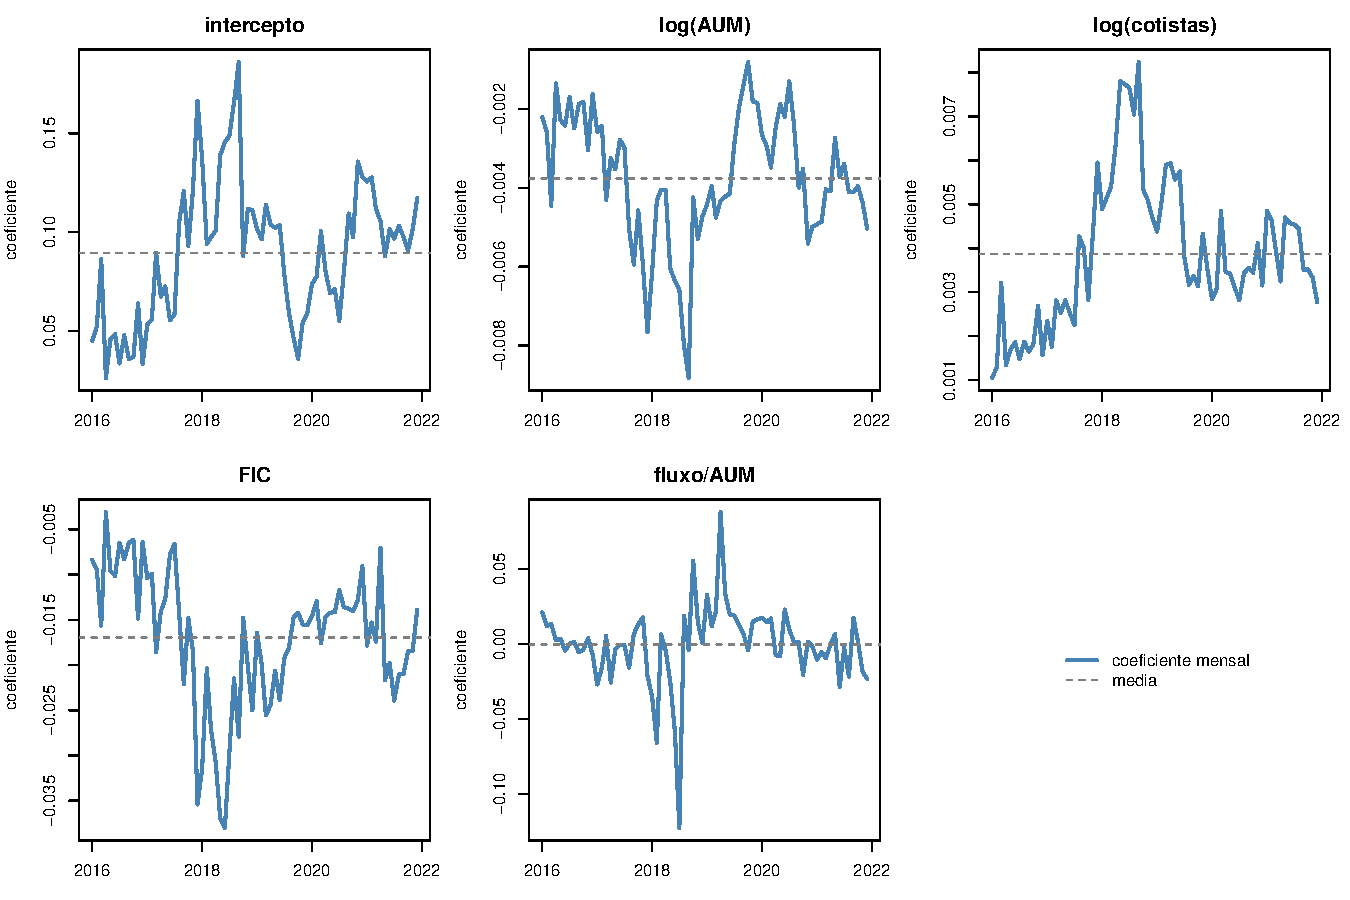
\includegraphics[width=0.86\textwidth]{fig_theta.pdf}
\caption{Coeficientes da regressão mês a mês, de 2016 a 2021. A linha tracejada marca a média de
cada série.}
\label{fig:theta}
\caption*{\footnotesize Fonte: elaboração própria.}
\end{figure}

A inspeção painel a painel da Figura~\ref{fig:theta} reforça e detalha essa leitura. No painel do
intercepto, a série parte de patamar baixo em 2016, sobe de forma acentuada até um pico em torno
de 2018 e depois recua, oscilando acima e abaixo da média da série; ou seja, o nível de referência
do peso não é constante, mas migra ao longo do tempo, o que é exatamente o tipo de variação suave
que justifica tratar o intercepto como estado latente. O painel de $\ln(\text{AUM})$ permanece
inteiramente abaixo de zero em todos os meses, confirmando a estabilidade do sinal negativo do
tamanho documentada na Tabela~\ref{tab:fmtab}, com oscilações que o tornam mais negativo por volta
de 2018 e menos negativo em janelas posteriores. O painel de $\ln(\text{cotistas})$ é o de
variação mais pronunciada: o coeficiente sobe fortemente até um máximo em torno de 2018 e depois
reverte, mas mantém-se positivo praticamente em todo o período, o que mostra que a associação
positiva entre número de cotistas e peso é persistente em sinal, ainda que variável em
intensidade. O painel de FIC é negativo em todos os meses, com um vale acentuado por volta de
2018, indicando que a penalidade de peso dos fundos de cotas se aprofunda nesse período e depois
se atenua, sem nunca mudar de sinal. Por fim, o painel de fluxo sobre patrimônio oscila em torno
de zero ao longo de quase toda a amostra, com um único movimento negativo isolado e profundo
próximo de 2018; esse comportamento, centrado em zero e dominado por um episódio extremo, é
coerente com a não significância da captação na Tabela~\ref{tab:fmtab} e sugere que o pico reflete
as caudas extremas da razão fluxo sobre patrimônio em fundos pequenos, e não um efeito
sistemático.

Dois pontos sintetizam a figura. Primeiro, todos os coeficientes de característica de fundo
preservam o sinal ao longo dos 72 meses, o que sustenta a estabilidade qualitativa afirmada na
Seção~\ref{sec:det}. Segundo, a concentração de movimentos em torno de 2018 em vários painéis,
intercepto, cotistas, FIC e fluxo, indica um período de reconfiguração comum das posições,
possivelmente ligado às condições de mercado da ação naquele intervalo, em que o preço e o beta
também se moveram de forma acentuada. Essa coincidência temporal motiva, na continuação, examinar
se há um fator comum por trás da variação simultânea dos coeficientes.

\subsection{Previsão e a matriz de erros}

O resultado de previsão é o mais surpreendente e está na Tabela~\ref{tab:fc}. Avaliando fora da
amostra, nenhum modelo estrutural supera a previsão ingênua de repetir o último peso. Acrescentar
um nível próprio de cada fundo, por meio de um efeito fixo, ou prever os coeficientes pelo filtro
de Kalman, piora a previsão; modelar diretamente a variação do peso apenas empata com a regra
ingênua. O fato de a média histórica do próprio fundo prever pior do que o último valor indica que
o peso não reverte a uma média no nível do fundo, e sim que é muito persistente, próximo de um
passeio aleatório. Os erros do melhor modelo têm média praticamente nula e formam uma série
estacionária, propriedades que se desejava verificar.

A leitura quantitativa da Tabela~\ref{tab:fc} torna o contraste nítido. No universo de todos os
fundos e horizonte de um mês, a raiz do erro quadrático médio da previsão ingênua é 0,0156, contra
0,0240 do nível do fundo e 0,0255 do fator com Kalman: os modelos estruturais erram cerca de 54 a
63 por cento mais do que a regra simples. O modelo de variação do peso iguala a regra ingênua,
0,0156, o que é coerente, pois prever variação nula equivale a repetir o último peso. Que o efeito
fixo de fundo, que captura o nível médio histórico, perca para o último valor é o ponto mais
revelador da tabela: ele mostra que não há reversão a uma média de fundo no curto prazo; se
houvesse, a média histórica bateria o último valor. O que se observa é o oposto, sinal de
persistência próxima do passeio aleatório.

\begin{table}[h]\centering\small
\caption{Erro de previsão fora da amostra, medido pela raiz do erro quadrático médio, nos
horizontes de um e de três meses.}
\label{tab:fc}
\begin{tabular}{@{}llrrrr@{}}
\toprule
Universo & Horizonte & Ingênua & Nível do fundo & Fator com Kalman & Variação do peso \\
\midrule
Todos os fundos      & 1 mês  & $0{,}0156$ & $0{,}0240$ & $0{,}0255$ & $0{,}0156$ \\
Todos os fundos      & 3 meses& $0{,}0207$ & $0{,}0262$ & $0{,}0273$ & $0{,}0210$ \\
Só fundos de ações   & 1 mês  & $0{,}0197$ & $0{,}0310$ & $0{,}0383$ & $0{,}0198$ \\
Só fundos de ações   & 3 meses& $0{,}0266$ & $0{,}0337$ & $0{,}0385$ & $0{,}0270$ \\
\bottomrule
\end{tabular}
\caption*{\footnotesize Fonte: elaboração própria.}
\end{table}

No horizonte de três meses a previsão ingênua piora, como era de esperar, passando de 0,0156 para
0,0207 no universo completo, e a distância para os modelos estruturais diminui, de modo que o
fator com Kalman vai de 0,0255 para 0,0273; ainda assim a regra ingênua vence em todas as linhas.
Restringir a amostra apenas aos fundos de ações não altera essa conclusão, apenas a torna mais
nítida, pois nesses fundos as posições em VALE3 são maiores e mais variáveis: os erros de todos os
métodos sobem, mas a ordem se mantém, com a ingênua em 0,0197 a um mês e 0,0266 a três meses,
sempre à frente. A leitura prudente é a de que, no curto prazo, a inércia do próprio fundo
constitui um teto difícil de superar, e que o modelo de fator deve ser visto, por ora, como
ferramenta de compreensão, e não de previsão. Vale notar que esse achado é exatamente o que o
modelo de ajuste parcial da Seção~\ref{sec:pa} antecipa no limite: se a velocidade de ajuste
$\lambda_n$ for próxima de zero, a melhor previsão é repetir o último peso, e a tabela é
consistente com esse regime.

\subsection{As duas margens}

Por fim, separa-se a decisão de ter a ação da decisão de quanto carregar. A regressão logística da
probabilidade de o fundo ter VALE3 revela um padrão que se considera o mais interessante do
trabalho: as duas decisões têm sinais opostos, como sintetiza a Tabela~\ref{tab:margens}. Fundos
maiores e fundos de cotas são mais propensos a ter a ação, mas, quando a têm, carregam um peso
menor. Esse padrão é compatível com diversificação, no sentido de que esses fundos espalham a
carteira por muitas ações, incluindo VALE3, cada uma com uma fatia pequena. A posse, por sua vez,
é ainda mais persistente que o peso, e novamente a previsão ingênua de repetir o estado anterior
acerta muito mais do que o modelo com características.

\begin{table}[h]\centering\small
\caption{Sinais opostos entre a decisão de ter a ação e a decisão de quanto carregar.}
\label{tab:margens}
\begin{tabular}{@{}lcc@{}}
\toprule
Característica & Ter ou não a ação & Quanto carregar \\
\midrule
Tamanho do fundo   & mais provável ter & peso menor \\
Fundo de cotas     & mais provável ter & peso menor \\
Número de cotistas & menos provável (efeito fraco) & peso maior \\
\bottomrule
\end{tabular}
\caption*{\footnotesize Fonte: elaboração própria.}
\end{table}

O contraste de sinais da Tabela~\ref{tab:margens} merece ser lido com o vocabulário de demanda. A
margem extensiva, ter ou não, e a margem intensiva, quanto carregar, respondem de forma oposta às
mesmas características de tamanho e de classificação de cotas. Para o tamanho e para fundo de
cotas, a probabilidade de incluir VALE3 cresce, enquanto o peso, condicional à inclusão, cai. Esse
é precisamente o padrão esperado de carteiras diversificadas: à medida que o fundo cresce ou
acessa o ativo de forma indireta, ele tende a incluir mais ativos, cada um com participação menor.
O número de cotistas exibe o sentido oposto nas duas margens, com efeito fraco na decisão de ter e
efeito positivo no peso, o que sugere que a dispersão de cotistas se associa a posições diretas
maiores quando elas existem. Como advertência metodológica, a separação formal dessas duas margens
pede, na continuação, um modelo em duas partes que trate de forma conjunta a decisão de posse e a
de peso, em vez de dois exercícios independentes.

%==================== 5. DISCUSSÃO ====================
\section{Discussão}

Este trabalho organizou, a partir das bases públicas da Comissão de Valores Mobiliários, um painel
mensal dos pesos da ação VALE3 nas carteiras dos fundos do grupo Itaú entre 2016 e 2021, e o
utilizou para responder a duas perguntas. A primeira era quais características de um fundo explicam
o peso que ele atribui à ação. A segunda era se esse peso pode ser previsto de um mês para o
outro. A evidência reunida sugere respostas claras e, em parte, contrastantes. O peso é bem
explicado pela seção transversal, por tamanho do fundo, número de cotistas, classificação de fundo
de cotas e beta da ação, com sinais estáveis ao longo de todo o período, conforme mostram as
Tabelas~\ref{tab:fmtab} e \ref{tab:pool} e a Figura~\ref{fig:theta}, e a decisão de ter a ação
carrega sinais opostos aos da decisão de quanto carregar, um padrão compatível com diversificação.
Para previsão, contudo, nenhum dos modelos estruturais testados supera a previsão ingênua de
repetir o último peso, mesmo sob a defasagem trimestral de divulgação das carteiras, de modo que o
peso se comporta, no nível do fundo, de forma muito persistente, próxima de um passeio aleatório,
como evidencia a Tabela~\ref{tab:fc}.

A interpretação que se extrai é que o fator latente é, antes de tudo, uma ferramenta de
compreensão, capaz de revelar quais características importam para as posições, e não um modelo de
previsão de curto prazo, território em que a inércia do próprio fundo domina. Esse achado deve ser
lido à luz de algumas limitações, várias delas já mapeadas para tratamento. A análise restringe-se
a uma única ação e a uma única gestora, em um período específico, de modo que a generalização
requer cautela. A leitura do coeficiente do beta como aversão a risco está contaminada pela
colinearidade entre preço e beta, e a separação entre efeito mecânico do preço e decisão ativa do
gestor ainda não foi feita. A variável de captação sobre patrimônio apresenta caudas extremas em
fundos de patrimônio muito pequeno, visíveis no painel de fluxo da Figura~\ref{fig:theta}, ainda
não tratadas. E o limiar de três cotistas usado para excluir fundos exclusivos é uma convenção
cuja sensibilidade resta documentar.

As limitações apontam diretamente para a agenda futura, centrada no modelo de ajuste parcial da
carteira especificado na Seção 3. O passo seguinte é estimar a velocidade de ajuste, com atenção
ao viés de atenuação discutido na Seção~\ref{sec:pa}: como a distância ao alvo é um regressor
medido com erro, a estimação deve usar variável instrumental ou correção de erros nas variáveis, e
não regularização do tipo \emph{ridge}, que agravaria a atenuação contra a hipótese de interesse.
O teste central será verificar se essa velocidade é estatisticamente diferente de zero e
caracterizar a série de erros de previsão sob a defasagem de divulgação. De forma complementar,
pretende-se estender a análise a outras ações e gestoras, aproveitando que o código construído é
facilmente adaptável; tratar as caudas extremas da variável de captação; decompor a parte do peso
que muda apenas em razão da variação do preço daquela que reflete decisão ativa; e modelar de
forma mais formal a margem extensiva por meio de um modelo em duas partes. Todo o código, os dados
e o registro das decisões metodológicas estão organizados no repositório público do
projeto\footnote{Disponível em \url{https://github.com/JoaoPauloZangrandi/forecasting-fund-weights-vale-itau}.},
de modo a tornar os resultados reprodutíveis.

%==================== REFERÊNCIAS ====================
\newpage
\addcontentsline{toc}{section}{Referências}
\section*{Referências}
\small
\begin{description}
\item Coval, Joshua and Erik Stafford. Asset fire sales (and purchases) in equity markets.
\emph{Journal of Financial Economics}, 86(2):479--512, 2007.
\item Fama, Eugene F. and James D. MacBeth. Risk, return, and equilibrium: empirical tests.
\emph{Journal of Political Economy}, 81(3):607--636, 1973.
\item Gabaix, Xavier and Ralph S. J. Koijen. In search of the origins of financial fluctuations:
the inelastic markets hypothesis. \emph{NBER Working Paper} 28967, 2021.
\item Harvey, Andrew C. \emph{Forecasting, Structural Time Series Models and the Kalman Filter}.
Cambridge University Press, Cambridge, 1989.
\item Hoerl, Arthur E. and Robert W. Kennard. Ridge regression: biased estimation for
nonorthogonal problems. \emph{Technometrics}, 12(1):55--67, 1970.
\item Koijen, Ralph S. J. and Motohiro Yogo. A demand system approach to asset pricing.
\emph{Journal of Political Economy}, 127(4):1475--1515, 2019.
\item Lou, Dong. A flow-based explanation for return predictability. \emph{Review of Financial
Studies}, 25(12):3457--3489, 2012.
\item Newey, Whitney K. and Kenneth D. West. A simple, positive semi-definite, heteroskedasticity
and autocorrelation consistent covariance matrix. \emph{Econometrica}, 55(3):703--708, 1987.
\item Papke, Leslie E. and Jeffrey M. Wooldridge. Econometric methods for fractional response
variables with an application to 401(k) plan participation rates. \emph{Journal of Applied
Econometrics}, 11(6):619--632, 1996.
\end{description}

\end{document}
